% !TEX TS-program = XeLaTeX
% use the following command: 
% all document files must be coded in UTF-8
\documentclass{textolivre}
% for anonymous submission
%\documentclass[anonymous]{textolivre}
% to create HTML use 
%\documentclass{textolivre-html}
% See more information on the repository: https://github.com/leolca/textolivre

% Metadata
\begin{filecontents*}[overwrite]{article.xmpdata}
    \Title{A intertextualidade em hipertextos: uma análise de tweets de cunho didático}
    \Author{Ana Claudia Oliveira Azevedo \sep Márcia Helena de Melo Pereira}
    \Language{pt-BR}
    \Keywords{Hipertexto \sep Intertextualidade \sep Tweet \sep Twitter}
    \Journaltitle{Texto Livre}
    \Journalnumber{1983-3652}
    \Volume{14}
    \Issue{3}
    \Firstpage{1}
    \Lastpage{16}
    \Doi{10.35699/1983-3652.2021.32557}

    \setRGBcolorprofile{sRGB_IEC61966-2-1_black_scaled.icc}
            {sRGB_IEC61966-2-1_black_scaled}
            {sRGB IEC61966 v2.1 with black scaling}
            {http://www.color.org}
\end{filecontents*}

% used to create dummy text for the template file
\definecolor{dark-gray}{gray}{0.35} % color used to display dummy texts
\usepackage{lipsum}
\SetLipsumParListSurrounders{\colorlet{oldcolor}{.}\color{dark-gray}}{\color{oldcolor}}

% used here only to provide the XeLaTeX and BibTeX logos
\usepackage{hologo}

% used in this example to provide source code environment
%\crefname{lstlisting}{lista}{listas}
%\Crefname{lstlisting}{Lista}{Listas}
%\usepackage{listings}
%\renewcommand\lstlistingname{Lista}
%\lstset{language=bash,
        breaklines=true,
        basicstyle=\linespread{1}\small\ttfamily,
        numbers=none,xleftmargin=0.5cm,
        frame=none,
        framexleftmargin=0.5em,
        framexrightmargin=0.5em,
        showstringspaces=false,
        upquote=true,
        commentstyle=\color{gray},
        literate=%
           {á}{{\'a}}1 {é}{{\'e}}1 {í}{{\'i}}1 {ó}{{\'o}}1 {ú}{{\'u}}1 
           {à}{{\`a}}1 {è}{{\`e}}1 {ì}{{\`i}}1 {ò}{{\`o}}1 {ù}{{\`u}}1
           {ã}{{\~a}}1 {ẽ}{{\~e}}1 {ĩ}{{\~i}}1 {õ}{{\~o}}1 {ũ}{{\~u}}1
           {â}{{\^a}}1 {ê}{{\^e}}1 {î}{{\^i}}1 {ô}{{\^o}}1 {û}{{\^u}}1
           {ä}{{\"a}}1 {ë}{{\"e}}1 {ï}{{\"i}}1 {ö}{{\"o}}1 {ü}{{\"u}}1
           {Á}{{\'A}}1 {É}{{\'E}}1 {Í}{{\'I}}1 {Ó}{{\'O}}1 {Ú}{{\'U}}1
           {À}{{\`A}}1 {È}{{\`E}}1 {Ì}{{\`I}}1 {Ò}{{\`O}}1 {Ù}{{\`U}}1
           {Ã}{{\~A}}1 {Ẽ}{{\~E}}1 {Ũ}{{\~u}}1 {Õ}{{\~O}}1 {Ũ}{{\~U}}1
           {Â}{{\^A}}1 {Ê}{{\^E}}1 {Î}{{\^I}}1 {Ô}{{\^O}}1 {Û}{{\^U}}1
           {Ä}{{\"A}}1 {Ë}{{\"E}}1 {Ï}{{\"I}}1 {Ö}{{\"O}}1 {Ü}{{\"U}}1
           {ç}{{\c{c}}}1 {Ç}{{\c{C}}}1
}


\journalname{Texto Livre}
\thevolume{14}
\thenumber{3}
\theyear{2021}
\receiveddate{\DTMdisplaydate{2021}{3}{17}{-1}} % YYYY MM DD
\accepteddate{\DTMdisplaydate{2021}{6}{14}{-1}}
\publisheddate{\DTMdisplaydate{2021}{8}{18}{-1}}
% Corresponding author
\corrauthor{Ana Claudia Oliveira Azevedo}
% DOI
\articledoi{10.35699/1983-3652.2021.32557}
%\articleid{NNNN} % if the article ID is not the last 5 numbers of its DOI, provide it using \articleid{} commmand
% list of available sesscions in the journal: articles, dossier, reports, essays, reviews, interviews, editorial
\articlesessionname{articles}
% Abbreviated author list for the running footer
\runningauthor{Azevedo e Pereira}
\sectioneditorname{Daniervelin Pereira}
\layouteditorname{Daniervelin Pereira}

\title{A intertextualidade em hipertextos: uma análise de \textit{tweets} de cunho didático}
\othertitle{Intertextuality in hypertexts: an analysis of didactic tweets}
% if there is a third language title, add here:
%\othertitle{Artikelvorlage zur Einreichung beim Texto Livre Journal}

\author[1]{Ana Claudia Oliveira Azevedo \orcid{0000-0002-8729-6515} \thanks{Email: \url{98anaclaudia@gmail.com}}}
\author[2]{Márcia Helena de Melo Pereira \orcid{0000-0002-3663-3462} \thanks{Email: \url{marciahelenad@yahoo.com.br}}}

%FALTA ORCID

\affil[1]{Universidade Estadual do Sudoeste da Bahia, Programa de Pós-Graduação em Linguística, Vitória da Conquista, BA, Brasil.}
\affil[2]{Universidade Estadual do Sudoeste da Bahia, Departamento de Estudos Linguísticos e Literários, Programa de Pós-Graduação em Linguística, Vitória da Conquista, BA, Brasil.}

\addbibresource{article.bib}
% use biber instead of bibtex
% $ biber tl-article-template

% set language of the article
\setdefaultlanguage[variant=brazilian]{portuguese}
\setotherlanguage{english}

% for spanish, use:
%\setdefaultlanguage{spanish}
%\gappto\captionsspanish{\renewcommand{\tablename}{Tabla}} % use 'Tabla' instead of 'Cuadro'
%\AfterEndPreamble{\crefname{table}{tabla}{tablas}\Crefname{table}{Tabla}{Tablas}}

% for languages that use special fonts, you must provide the typeface that will be used
% \setotherlanguage{arabic}
% \newfontfamily\arabicfont[Script=Arabic]{Amiri}
% \newfontfamily\arabicfontsf[Script=Arabic]{Amiri}
% \newfontfamily\arabicfonttt[Script=Arabic]{Amiri}
%
% in the article, to add arabic text use: \textlang{arabic}{ ... }

% for russian text we also need to define fonts with support for Cyrillic script
% \usepackage{fontspec}
% \setotherlanguage{russian}
% \newfontfamily\cyrillicfont{Times New Roman}
% \newfontfamily\cyrillicfontsf{Times New Roman}[Script=Cyrillic]
% \newfontfamily\cyrillicfonttt{Times New Roman}[Script=Cyrillic]
%
% in the text use \begin{russian} ... \end{russian}

% to use emoticons in your manuscript
% https://stackoverflow.com/questions/190145/how-to-insert-emoticons-in-latex/57076064
% using font Symbola, which has full support
% the font may be downloaded at:
% https://dn-works.com/ufas/
% add to preamble:
% \newfontfamily\Symbola{Symbola}
% in the text use:
% {\Symbola }

% reference itens in a descriptive list using their labels instead of numbers
% insert the code below in the preambule:
\makeatletter
\let\orgdescriptionlabel\descriptionlabel
\renewcommand*{\descriptionlabel}[1]{%
  \let\orglabel\label
  \let\label\@gobble
  \phantomsection
  \edef\@currentlabel{#1\unskip}%
  \let\label\orglabel
  \orgdescriptionlabel{#1}%
}
\makeatother
%
% in your document, use as illustraded here:
%\begin{description}
%  \item[first\label{itm1}] this is only an example;
%  % ...  add more items
%\end{description}
 

% custom epigraph - BEGIN 
%%% https://tex.stackexchange.com/questions/193178/specific-epigraph-style
\usepackage{epigraph}
\renewcommand\textflush{flushright}
\makeatletter
\newlength\epitextskip
\pretocmd{\@epitext}{\em}{}{}
\apptocmd{\@epitext}{\em}{}{}
\patchcmd{\epigraph}{\@epitext{#1}\\}{\@epitext{#1}\\[\epitextskip]}{}{}
\makeatother
\setlength\epigraphrule{0pt}
\setlength\epitextskip{0.5ex}
\setlength\epigraphwidth{.7\textwidth}
% custom epigraph - END


% if you use multirows in a table, include the multirow package
\usepackage{multirow}

% add line numbers for submission
%\usepackage{lineno}
%\linenumbers

\begin{document}
\maketitle

\begin{polyabstract}
\begin{abstract}
O objetivo deste artigo é analisar diferentes categorias do fenômeno de intertextualidade em tweets de cunho didático. O termo “intertextualidade”, que está relacionado ao conceito bakhtiniano de dialogismo, vem da teoria literária e é usado para se referir ao diálogo entre textos, tanto em sentido restrito quanto em sentido amplo. Trata-se de um aspecto comum a todos os textos, inclusive nos textos da internet, isto é, nos hipertextos, caracterizados, dentre outros aspectos, por um alto grau de multimodalidade. Neste artigo, foram observados os tipos de intertextualidade elencados por \textcite{koch_intertextualidade:_2012} em quatro (hiper)textos do gênero tweet que abordam conteúdos didáticos de diferentes áreas do conhecimento — Ciências Naturais, Ciências Humanas, Linguagens e Matemática —, coletados por meio de capturas de tela. A análise mostrou que diversas categorias de intertextualidade ocorrem produtivamente em (hiper)textos do gênero tweet, o que confirma o pressuposto de que esse fenômeno é constitutivo da linguagem. Além disso, constatou-se que a intertextualidade não se dá apenas no âmbito verbal, considerando que o tweet, por ser um hipertexto, permite a convergência de linguagens.

\keywords{Hipertexto \sep Intertextualidade \sep Tweet \sep Twitter}
\end{abstract}

\begin{english}
\begin{abstract}
The objective of this article is to analyze different categories of the intertextuality phenomenon in didactic tweets. The term “intertextuality”, which is related to the Bakhtinian concept of dialogism, comes from the literary theory and is used to refer to the dialogue between texts, both in a strict and in a wide sense. This is a common aspect to all the texts, including internet texts, that is, hypertexts, characterized, among other aspects, by a high degree of multimodality. In this article, the types of intertextuality listed by \textcite{koch_intertextualidade:_2012} were observed in four (hyper)texts of the tweet genre. These tweets approach educational contents from different areas of knowledge — Natural Sciences, Human Sciences, Languages, and Mathematics — and were collected through screenshots. The analysis showed that several categories of intertextuality occur productively in (hyper)texts of the tweet genre, which confirms the assumption that this phenomenon is constitutive of the language. Moreover, it was found that intertextuality does not occur only verbally, since the tweet, as a hypertext, allows the convergence of languages.

\keywords{Hypertext \sep Intertextuality \sep Tweet \sep Twitter}
\end{abstract}
\end{english}

% if there is another abstract, insert it here using the same scheme
\end{polyabstract}


\section{Introdução}\label{sec-intro}
Uma das principais discussões da teoria construída pelo Círculo de Bakhtin é a questão do dialogismo. Segundo \textcite{bakhtin_os_2011}, a comunicação humana é efetivada por meio do diálogo entre dois sujeitos, que alternam as posições ativas de falante e ouvinte. Além disso, o teórico aponta que nosso discurso “[…] é pleno de palavras dos outros, de um grau vário de alteridade ou de assimilabilidade, de um grau vário de aperceptibilidade e de relevância” \cite[p. 294-295]{bakhtin_os_2011}. Ou seja, a comunicação humana é permeada pelo diálogo entre sujeitos e pelo diálogo entre discursos, que se dá sempre por meio de gêneros do discurso, os quais ocorrem nos mais variados campos da atividade humana.

O diálogo entre discursos ou entre textos\footnote{Para \textcite{araujo_consideracoes_2009}, abordar os diálogos entre discursos permite uma análise mais ampla do que a abordagem do diálogo entre textos. No entanto, considerando que a relação entre texto e discurso é bastante próxima, uma vez que este é materializado naquele, entendemos que o diálogo entre textos inclui o diálogo entre discursos e vice-e-versa.} foi denominado, na área da teoria literária, de \textit{intertextualidade} \cite{kristeva_introducao_2005}. Posteriormente, o conceito foi apropriado pela Linguística Textual (doravante LT) e tem sido usado, até então, para se referir às relações estabelecidas entre textos de diversos campos da atividade humana. Autores como \textcite{koch__1991, koch_coerencia_2015, koch_intertextualidade:_2012} apresentam formas de categorização da intertextualidade que levam em conta aspectos como a (não) menção explícita do texto-fonte, a relação temática e estilística entre textos, além de outros fatores, sobre os quais discorreremos mais detalhadamente adiante.

A intertextualidade é considerada por linguistas como \textcite{koch_coerencia_2015} como um fator de coerência textual. Além disso, de acordo com \textcite{xavier_desafio_2015}, é, também, uma característica básica do hipertexto\footnote{Neste trabalho, utilizamos o termo “hipertexto” em sentido mais restrito, para fazer referência aos textos digitais disponíveis na internet.}, definido pelo autor como um dispositivo textual que proporciona a intersecção entre diferentes linguagens (verbal, visual e sonora) na internet. Ou seja, o fenômeno de intertextualidade está presente em todos os textos; no entanto, no hipertexto, apresenta determinadas particularidades, as quais tornam importante a sua investigação de modo mais específico. Dentre essas particularidades, ressaltamos a multimodalidade/multissemiose\footnote{Apesar de compreendermos que os conceitos de multimodalidade e multissemiose têm origem em diferentes vertentes teóricas, consideramos, com base em \textcite[p. 108]{rojo_hipermodernidade_2015}, que “texto multimodal ou multissemiótico é aquele que recorre a mais de uma modalidade de linguagem ou a mais de um sistema de signos ou símbolos (semiose) em sua composição”.}, que, conforme \textcite{garcia_intertextualidade_2020}, faz com que as pistas intertextuais, especialmente nos textos publicados em ambiente digital, não se limitem à linguagem verbal.

Nesse sentido, é importante ressaltar que \textcite{araujo_consideracoes_2009} criticam o fato de a intertextualidade no hipertexto ser, em muitas análises, limitada ao mero uso de \textit{links}, o que reduz o conceito apenas à indicação direta do intertexto. Então, os autores destacam que a investigação do fenômeno de intertextualidade no hipertexto “[…] se mostrará mais produtiva se, a exemplo do que se tem feito no âmbito da linguística textual, procedermos a uma análise mais criteriosa, seja em sentido restrito, seja em sentido amplo, considerando as relações estabelecidas pelos \textit{hiperlinks}” \cite[p. 579, grifo dos autores]{araujo_consideracoes_2009}. É o que nos propomos a fazer no presente artigo.

Portanto, neste trabalho, buscamos investigar o fenômeno de intertextualidade em (hiper)textos do gênero \textit{tweet}, produzidos e publicados na rede social Twitter, a fim de demonstrar, de modo mais detalhado, o funcionamento dessa categoria em um gênero discursivo digital. Nosso corpus é formado por capturas de tela de tweets que dialogam com assuntos escolares das áreas de Ciências Naturais, Ciências Humanas, Linguagens e Matemática.

Na próxima seção, apresentamos pressupostos teóricos acerca do gênero a ser analisado, o \textit{tweet}, levando em consideração a teoria bakhtiniana de gêneros discursivos e as particularidades do hipertexto. Em seguida, na \cref{sec-conduta}, discorremos a respeito da intertextualidade e suas categorizações, ressaltando que esse fenômeno ocorre, também, por meio de elementos de linguagem não verbal. Posteriormente, na \cref{sec-fmt-manuscrito}, explicamos brevemente a metodologia de coleta do \textit{corpus} e, logo depois, exibimos os resultados e discussão da análise dos dados. Por fim, na \cref{sec-formato}, realizamos as considerações finais do trabalho.

\section{O gênero discursivo tweet: hipertexto de até 280 caracteres}\label{sec-normas}
De acordo com \textcite{bakhtin_os_2011}, a comunicação humana, em diferentes campos, ocorre sempre por meio de \textit{tipos relativamente estáveis de enunciados}, nomeados por ele de gêneros do discurso. O teórico afirma que a relativa estabilidade dos gêneros é observável em sua construção composicional, estilo e conteúdo temático, pilares que compõem todos os gêneros do discurso que circulam na sociedade.

A construção composicional compreende, basicamente, a organização e a (macro)estrutura do enunciado, que diferenciam o seu formato do de outros gêneros. O estilo, por sua vez, é constituído pelas escolhas linguísticas feitas para dizer o que se pretende. Para \textcite{bakhtin_os_2011}, além do estilo linguístico (do gênero), existe o estilo individual (do autor), o qual é representado por intervenções particulares\footnote{Vale ressaltar que, para \textcite{bakhtin_os_2011}, o sujeito sempre enuncia de dentro de um campo da atividade humana, que lhe impõe certos limites e direções, visto que está situado em determinadas condições sócio-histórico-culturais. Portanto, o sujeito não é totalmente assujeitado nem totalmente dono de seu dizer.} no gênero e é mais passível de ocorrer em gêneros menos padronizados, cujo estilo é mais flexível. Por fim, o conteúdo temático consiste na apreciação valorativa do falante sobre determinado assunto, a qual está, também, determinada socio-historicamente e, logo, relacionada ao campo da atividade humana do qual o sujeito faz parte. Segundo \textcite{bakhtin_os_2011}, os três pilares integrantes do gênero estão interligados e são essenciais para sua caracterização.

O desenvolvimento tecnológico das novas mídias, mais especificamente da internet, ocasionou novos gêneros do discurso, que se materializam em hipertextos. Conforme \textcite{xavier_desafio_2015}, o termo “hipertexto” foi cunhado, no final dos anos 1960, por Ted Nelson, para se referir a um sistema de escrita cujo funcionamento se assemelharia ao modo de pensar humano, que conecta informações de modo não sequencial. Posteriormente, com a popularização da internet, o hipertexto, como idealizado pelo norte-americano, tornou-se tecnologicamente possível e tem sido usado nos mais diferentes campos da comunicação humana.

\textcite{araujo_consideracoes_2009} definem o hipertexto como um modo de enunciar que apresenta possibilidades além das permitidas pelo papel, visto que mescla diversos modos enunciativos (palavras, imagens e sons). Então, assim como os linguistas, adotamos uma definição mais estrita de hipertexto, observando as especificidades do “[…] ‘texto da internet’ no qual se encontram palavras, imagens, vídeos e sonoridades todos passíveis de percepção simultânea, co-ocorrendo sem concorrer, uma vez que todos os modos enunciativos colaboram para a produção de sentido” \cite[p. 79]{xavier_desafio_2015}. Vejamos, a seguir, os cinco principais aspectos que, segundo \textcite{xavier_desafio_2015}, caracterizam o hipertexto on-line e o particularizam em relação ao texto impresso ou manuscrito.

A primeira característica elencada por \textcite{xavier_desafio_2015} é a \textit{imaterialidade/virtualidade}, uma vez que o hipertexto só pode ser acessado virtualmente, e não fisicamente; logo, quando impresso, perde a virtualidade. A segunda característica é a \textit{ubiquidade}, pois o acesso ao hipertexto pode ocorrer simultaneamente de vários lugares, em qualquer momento, por qualquer pessoa que esteja conectada à internet; ao contrário do texto impresso/manuscrito, que só pode ser lido por alguém que esteja no mesmo tempo e espaço físico que ele. O terceiro elemento que compõe o hipertexto, conforme \textcite{xavier_desafio_2015}, é a \textit{convergência de linguagens e mídias}, visto que os diferentes modos de enunciação (verbal, visual e sonoro) coocorrem no hipertexto, gerando um novo modo de enunciação: o digital. A quarta característica do hipertexto é a \textit{não-linearidade} constitutiva, que é levada em consideração desde o momento de produção do hipertexto e exige habilidades específicas do leitor para a sua compreensão. A última característica apresentada por \textcite{xavier_desafio_2015} é a \textit{intertextualidade infinita}, tendo em vista que a internet potencializa a inter-relação entre dizeres e, assim, “a intertextualidade chega ao seu apogeu, posto que todos os hipertextos por princípio se cruzam na Internet” \cite[p. 82]{xavier_desafio_2015}. Esse último aspecto será observado mais de perto nas próximas seções deste trabalho.

Com base nessas assertivas, classificamos o \textit{tweet} como um gênero discursivo digital, isto é, um gênero do discurso produzido em ambiente \textit{on-line}, o que o categoriza como um hipertexto. Tendo em vista que a produção textual-discursiva na internet é caracterizada pelos cinco aspectos acima elencados, descrevemos o gênero específico investigado neste trabalho. O \textit{tweet} é, grosso modo, um texto de até 280 caracteres produzido na rede social Twitter, em tese, em resposta à pergunta “O que está acontecendo?”, feita na própria plataforma no momento de sua publicação. Apesar de apresentar diversas possibilidades a depender de quem o publica, o \textit{tweet} é considerado um gênero do discurso, como apontam \textcite{freitas_genero_2015} e \textcite{azevedo_o_2021}, uma vez que apresenta uma relativa estabilidade em sua construção composicional, estilo e conteúdo temático, sobre os quais discorreremos a seguir.

De acordo com \textcite{azevedo_o_2021}, a construção composicional do \textit{tweet} é marcada pela limitação de 280 caracteres escritos, que exige do seu produtor a manipulação de estratégias de sumarização e de adequação a esse limite, tais como o uso de abreviações, \textit{links}, vídeos, imagens, \textit{GIFs}\footnote{\textit{Graphic Interchange Format} — ou simplesmente \textit{GIF} — é um formato de imagem, geralmente com figuras em movimento.}, \textit{threads}\footnote{Nome dado a uma sequência de \textit{tweets} interligados, geralmente sobre o mesmo assunto.} etc., como mostram \textcite{azevedo_estrategias_2020}. No entanto, \textcite{azevedo_o_2021} apontam que, além desses aspectos, que podem ser escolhidos pelo produtor do \textit{tweet}, a estrutura do gênero — que o torna socialmente reconhecível — também é composta pela foto de perfil do usuário, o \textit{nickname} (apelido do usuário) e o \textit{user} (identificação particular de cada perfil, introduzida pelo símbolo @), acima do texto, e, na parte inferior, por data e horário de publicação, tipo de dispositivo por meio do qual o \textit{tweet} foi publicado (Android, iPhone, Web ou algum \textit{software} específico de publicação de \textit{tweets}) e \textit{links} de interação próprios da rede social Twitter (responder, \textit{retweetar}, curtir e salvar/compartilhar).

O estilo dos \textit{tweets}, por sua vez, é variável e está relacionado aos objetivos interacionais do perfil que os publica. Ainda assim, podemos mencionar a multimodalidade (uso de \textit{hashtags}, \textit{emojis}, \textit{links}, fotos, vídeos, \textit{GIFs} etc.) e a intertextualidade \cite{barth_letramento_2014} como fatores que podem constituir o estilo do gênero. Além disso, é comum que o \textit{tweet} apresente características de outros gêneros, que são reelaborados na sua constituição, tais como notícia, bilhete, conversa informal, citação \cite{freitas_genero_2015}, entre outros. Portanto, consideramos o \textit{tweet} como um gênero altamente flexível e aberto à inserção de estilo individual, que, de acordo com \textcite{barth_letramento_2014}, é marcado por escolhas pontuais dos usuários.

Além disso, o conteúdo temático dos tweets pode ser bem diverso, uma vez que, como defendem \textcite{freitas_genero_2015}, “um usuário comum pode tratar de uma gama ilimitada de assuntos. Porém, um usuário que representa uma entidade ou um usuário que representa uma empresa possui uma limitação temática”. Ou seja, o conteúdo temático dos tweets varia a depender dos propósitos e do perfil de cada usuário. Consequentemente, conforme \textcite{azevedo_o_2021}, os outros pilares do gênero também variam, uma vez que o conteúdo temático é responsável por direcionar a comunicação discursiva e determinar os aspectos linguísticos e composicionais de um enunciado, de modo que conteúdo temático, estilo e construção composicional estão interligados \cite{bakhtin_os_2011}.

Sendo assim, defendemos que o \textit{tweet} é um gênero do discurso, já que se trata de uma forma relativamente estável de enunciar, cujos recursos hipertextuais mobilizados variam de acordo com os objetivos e o estilo de cada usuário. Além disso, os aspectos sobre os quais comentamos ajudam a classificar o \textit{tweet} como hipertexto, uma vez que ele é produzido e acessível em ambiente virtual, portanto, é imaterial; é ubíquo — pode ser acessado simultaneamente por várias pessoas, em diferentes momentos e lugares —; é altamente multimodal/multissemiótico — tendo em vista a possibilidade de vincular outras linguagens à modalidade verbal escrita —; é constitutivamente não linear — sua formação é permeada por \textit{hiperlinks} e outros elementos que não são colocados de forma linear — e é intertextual, pois apresenta relações com outros textos. O fenômeno de intertextualidade, principal foco deste artigo, será abordado mais detalhadamente na próxima seção, na qual apresentamos um breve percurso do conceito, de modo a mostrar as categorias que serão levadas em consideração para a análise dos dados.

\section{Intertextualidade}\label{sec-conduta}
O termo intertextualidade foi inaugurado na área da teoria literária, mas, segundo \textcite{kristeva_introducao_2005}, criadora do conceito, tem uma relação próxima com o chamado dialogismo bakhtiniano. \textcite{bezerra_prefacio:_2018}, no prefácio ao livro \textit{Problemas da Poética de Dostoiévski}, traduzido por ele, critica a leitura da obra de Bakhtin por Kristeva. Segundo o tradutor, a teórica da literatura faz uma substituição terminológica equivocada de um “conceito-chave da teoria bakhtiniana do dialogismo” \cite[p. XIII]{bezerra_prefacio:_2018}, ao trocar \textit{palavra} por \textit{texto} e, consequentemente, \textit{dialogismo} por \textit{intertextualidade}. Com isso, de acordo com \textcite{bezerra_prefacio:_2018}, Kristeva produz um reducionismo da obra bakhtiniana, dando a ela um enfoque meramente linguístico e ignorando questões importantes da teoria de Bakhtin, como o diálogo entre vozes e a posição ativa dos sujeitos. Neste trabalho, embora reconheçamos possíveis equívocos da construção do conceito de \textit{intertextualidade} por sua criadora, acreditamos que a LT — cujas discussões serão apresentadas adiante — aborda a categoria com propriedade e oferece subsídios para um tratamento adequado do fenômeno, levando em consideração os postulados do Círculo de Bakhtin.

Nesse sentido, é importante apresentar brevemente alguns pressupostos do dialogismo bakhtiniano, para, em seguida, mostrar a construção do conceito de \textit{intertextualidade} na LT. \textcite[p. 298, grifos do autor]{bakhtin_os_2011}, ao eleger o enunciado como unidade real da comunicação, destaca que 

\begin{quote}
    o enunciado é pleno de \textit{tonalidades dialógicas} […] a nossa própria ideia – seja filosófica, científica, artística – nasce e se forma no processo de interação e luta com os pensamentos dos outros, e isso não pode deixar de encontrar o seu reflexo também nas formas de expressão verbalizada do nosso pensamento.
\end{quote}

Ou seja, os discursos de alguém sempre dialogam com discursos alheios, anteriores a ele, visto que nenhum discurso parte do nada. Desse modo, o teórico considera que, por meio da interação, em diversos gêneros do discurso, ocorre o diálogo — de forma direta ou indireta — com enunciados anteriores àqueles, bem como há abertura para a produção de enunciados futuros.

As concepções do Círculo de Bakhtin, datadas da primeira metade do século XX\footnote{Apesar de terem sido escritas majoritariamente entre as décadas de 1920 e 1960, as obras do Círculo de Bakhtin ganharam mais vigor a partir da segunda metade do século XX, quando foram redescobertas e reformuladas.}, foram retomadas e, como já mencionamos, adaptadas, à sua maneira, pela teórica da literatura Julia Kristeva. Em 1969, a autora cunhou o termo intertextualidade para se referir à relação entre textos, considerando que “todo texto se constrói como mosaico de citações, todo texto é absorção e transformação de um outro texto” \cite[p. 68]{kristeva_introducao_2005}. Anos depois, o conceito foi adotado pela LT, tendo em vista que o diálogo entre discursos/textos está presente não só em produções literárias, mas em gêneros dos mais diversos campos da atividade humana. Portanto, como apontam \textcite{araujo_consideracoes_2009}, a intertextualidade é um fenômeno constitutivo da linguagem humana.

Com base nisso, apresentamos, a seguir, algumas discussões realizadas pela LT ao longo dos anos, de modo a mostrar que as categorias de intertextualidade sofreram algumas modificações na área, conforme os estudos se desenvolveram. Então, discorremos acerca das perspectivas adotadas por \textcite{koch_coerencia_2015}, no livro \textit{A coerência textual}; por \textcite{koch__1991}, no artigo “Intertextualidade e polifonia: um só fenômeno?”; e por \textcite{koch_intertextualidade:_2012}, no livro \textit{Intertextualidade: diálogos possíveis}. Além disso, expomos os pressupostos de \textcite{mozdzenski_intertextualidade_2013, cavalcante_sobre_2017, garcia_intertextualidade_2020} acerca da ampliação do conceito de intertextualidade e sua aplicação a textos multissemióticos.

No livro \textit{A coerência textual}, publicado pela primeira vez em 1990, \textcite[p. 92]{koch_coerencia_2015}, ao defenderem que “para o processamento cognitivo (produção/recepção) de um texto recorre-se ao conhecimento prévio de outros textos”, elegem a intertextualidade como um dos fatores de coerência\footnote{\textcite{koch__1991} ressalta que Beaugrande e Dressler (1981) já haviam feito isso, ao elencarem a intertextualidade como um dos fatores de textualidade. Ou seja, a intertextualidade é um dos elementos essenciais para que determinada configuração linguística seja considerada um texto e, portanto, seja interpretável pelos leitores.}. Ou seja, para os linguistas, a intertextualidade é um elemento essencial para que determinada produção linguística faça sentido, visto que os textos que fazem parte do nosso conhecimento de mundo auxiliam na interpretação de novos textos, que têm relações com eles.

De acordo com \textcite{koch_coerencia_2015}, a intertextualidade pode ser de forma ou de conteúdo. Segundo os autores, “a intertextualidade de forma ocorre quando o produtor de um texto repete expressões, enunciados ou trechos de outros textos, ou então o estilo de determinado autor ou determinados gêneros do discurso” \cite[p. 92]{koch_coerencia_2015}. Essa categoria está ligada, portanto, à relação de estilo estabelecida por dois ou mais textos. Os linguistas acrescentam que a intertextualidade tipológica é um subtipo da intertextualidade formal e consiste no uso de superestruturas ou esquemas textuais que ficam armazenados na memória. Desse modo, “o conhecimento dos tipos textuais, portanto, permitirá ao leitor ‘enquadrar’ o texto em determinado esquema […]” \cite[p. 94]{koch_coerencia_2015}.

A intertextualidade de conteúdo, por sua vez, é considerada uma constante, visto que os textos de uma cultura sempre dialogam uns com os outros. Conforme \textcite{koch_coerencia_2015}, essa categoria de intertextualidade pode ocorrer de forma explícita — quando há indicação do texto-fonte — ou implícita — quando essa indicação não é feita, o que exige que o leitor ative seu conhecimento de mundo para identificar o texto de origem. Os autores comentam, ainda, a respeito da intertextualidade das semelhanças e da intertextualidade das diferenças, com base em Sant’Anna (1985), as quais dizem respeito, respectivamente, à adesão da ideia defendida no texto original e à oposição ao que é dito no texto-fonte.

Posteriormente, em um artigo publicado no ano de 1991, \textcite[p. 539]{koch__1991} defende que “a alteridade é necessariamente atestada pela presença de um intertexto, cuja fonte é explicitamente mencionada no texto que o incorpora ou cujo produtor está presente, em situações de comunicação oral”, uma vez que o intertexto deve fazer parte de “[…] um repertório partilhado por uma comunidade de fala”. Desse modo, vemos que a intertextualidade, como já comentamos, está estritamente relacionada ao dialogismo, que pressupõe o diálogo entre sujeitos e entre discursos, em determinadas condições socio-histórico-culturais.

A partir disso, a linguista apresenta algumas categorias de intertextualidade. Na primeira delas, divide a intertextualidade em sentido amplo — “[…] condição de existência do próprio discurso […]” \cite[p. 530]{koch__1991}, levando em consideração a sua heterogeneidade constitutiva, visto que todo discurso e todo texto dialogam com outros — e em sentido estrito — que se refere à relação com textos previamente existentes, efetivamente produzidos. A intertextualidade em sentido estrito é desmembrada em quatro grupos: 1) de conteúdo ou de forma e conteúdo; 2) explícita ou implícita; 3) das semelhanças ou das diferenças e 4) com intertexto alheio, com intertexto próprio ou com intertexto atribuído a um enunciador genérico.

No primeiro grupo, a linguista descarta a possibilidade de uma intertextualidade apenas de forma, uma vez que “[…] toda forma amolda/emoldura um conteúdo” \cite[p. 532]{koch__1991}. Com isso, opõe-se ao que defendera no livro \textit{A coerência textual}, no ano anterior. A intertextualidade de conteúdo, segundo \textcite{koch__1991}, ocorre, geralmente, entre textos de uma mesma área ou tendência do conhecimento, que compartilham termos específicos. A intertextualidade de forma e conteúdo, por sua vez, é caracterizada pela paródia da linguagem de textos já existentes, visando algum efeito específico. Em relação ao segundo grupo, \textcite{koch__1991} explica que a intertextualidade explícita se dá quando a fonte do intertexto é evidenciada, e a implícita, quando não há menção expressa ao texto-base. A intertextualidade das semelhanças e das diferenças, baseada em Sant’Anna (1985), diz respeito à orientação argumentativa dada ao texto-base, visto que o falante pode concordar com ele e usá-lo como argumento de autoridade ou refutá-lo de alguma forma. Por fim, a autora comenta que o texto pode ter relação com um intertexto alheio, próprio ou atribuído a um enunciador genérico.

Essas considerações são retomadas no livro \textit{Intertextualidade: diálogos possíveis}, de \textcite{koch_intertextualidade:_2012}. Nessa obra, as autoras apresentam uma tipologia mais detalhada para a classificação da intertextualidade, dividindo-a em: 1) intertextualidade \textit{stricto sensu}, que se subdivide em a) intertextualidade temática, b) intertextualidade estilística, c) intertextualidade explícita e d) intertextualidade implícita — a qual inclui o 2) \textit{détournement} —; 3) intertextualidade intergenérica; 4) intertextualidade tipológica; e 5) intertextualidade \textit{lato sensu}. As autoras comentam, ainda, sobre a relação entre intertextualidade e polifonia\footnote{De acordo com \textcite{koch_intertextualidade:_2012}, a polifonia consiste na copresença de vozes (pontos de vista) em um mesmo texto, ao passo que a intertextualidade diz respeito à presença de outros textos em um texto. Para as linguistas, “[…] há, entre intertextualidade e polifonia, uma relação de inclusão: a polifonia engloba todos os casos de intertextualidade, mas seu espectro é bem mais amplo que o daquela” \cite[p. 83]{koch_intertextualidade:_2012}. Assim, apesar de se tratar de coisas diferentes, ambos os fenômenos são manifestações da presença do outro em nossos discursos, como propõe Bakhtin ao comentar sobre o dialogismo.}, que não será abordada neste trabalho, visto que nosso foco são as categorias de intertextualidade propriamente ditas.

De acordo com \textcite{koch_intertextualidade:_2012}, a intertextualidade \textit{stricto sensu} consiste na retomada, em um novo texto, de (fragmentos de) textos efetivamente existentes, que fazem parte da memória social coletiva de determinada cultura e da memória discursiva individual dos falantes. Trata-se, então, da menção a um (ou mais) texto(s) específico(s), reconhecido(s) em um dado contexto socio-histórico-cultural. Esse tipo de intertextualidade pode se dar de diferentes formas, sobre as quais discorreremos a seguir.

A \textit{intertextualidade temática} ocorre quando um texto compartilha conceitos, nomenclaturas e terminologias com outros textos do mesmo campo. A \textit{intertextualidade estilística}, por sua vez, corresponde à reprodução voluntária de estilos, isto é, da linguagem de outros textos, com o intuito de fazer uma repetição, imitação ou paródia deles, para alcançar objetivos diversos. As autoras, assim como \textcite{koch__1991}, desconsideram a existência de uma intertextualidade apenas de forma, tendo em vista que toda forma emoldura um conteúdo. Com base nessa diversidade de objetivos que podem ser buscados pelos falantes, \textcite{mozdzenski_intertextualidade_2013} destaca que a função de ocorrência da intertextualidade deve ser considerada em um contínuo, tendo em vista os diferentes graus de aproximação e distanciamento da voz do autor do texto-fonte. Dentro desse contínuo, é possível encontrar desde uma citação “negativa” — na qual há uma desqualificação da voz do autor do texto-fonte — até uma citação “positiva” — em que se adota um ponto de vista próximo do autor do texto-fonte, por meio da autorização de sua voz —, além de paráfrase “negativa”, paródia/sátira, ironia, pastiche e paráfrase “positiva”.

Conforme \textcite{koch_intertextualidade:_2012}, a intertextualidade pode ser, ainda, \textit{explícita} — quando a fonte do intertexto, que pode ser um enunciador específico ou generalizado, é apontada — ou \textit{implícita} — quando não há menção à fonte. No caso da intertextualidade implícita, a alusão ao intertexto pode se dar por meio de paráfrases, que podem estar mais ou menos próximas do texto-fonte, ou de “[…] enunciados parodísticos e/ou irônicos, apropriações, reformulações de tipo concessivo, inversão da polaridade afirmação/negação, entre outros” \cite[p. 31]{koch_intertextualidade:_2012}. O plágio seria mais um tipo de intertextualidade implícita; no entanto, nesse caso, o produtor do texto espera que não haja recuperação da fonte. Nos outros dois casos, a identificação do intertexto implícito e a construção de um sentido próximo ao pretendido pelo produtor do texto são desejáveis e dependem da ativação da memória discursiva do leitor/ouvinte para seu reconhecimento; portanto, a depender do texto-fonte, há menos garantia de que esse reconhecimento ocorra. Consequentemente, segundo as autoras, “a não depreensão do texto-fonte, nesses casos, empobrece a leitura ou praticamente impossibilita a construção de sentidos próximos àqueles previstos na proposta de sentido do locutor” \cite[p. 36]{koch_intertextualidade:_2012}. 

\textcite{koch_intertextualidade:_2012} propõem, ainda, que seja mais adequado considerar diferentes graus de explicitude, identificáveis por meio de marcas linguísticas. Fundamentado nisso, \textcite{mozdzenski_intertextualidade_2013} elabora um contínuo tipológico relacionado à forma de ocorrência da intertextualidade, a fim de ampliar a concepção de graus de explicitude/implicitude, partindo, então, de um ponto de vista não dicotômico:

\begin{figure}[htbp]
 \centering
 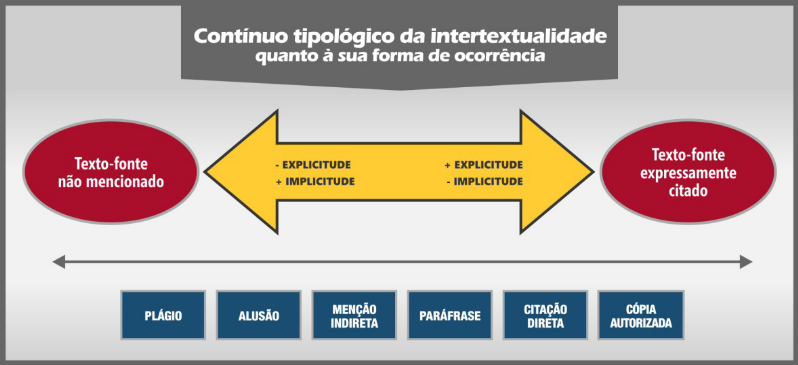
\includegraphics[width=0.85\textwidth]{Fig1.png}
 \caption{Contínuo tipológico da intertextualidade quanto à sua forma de ocorrência.}
 \label{fig01}
 \source{\textcite[p. 183]{mozdzenski_intertextualidade_2013}.}
\end{figure}

Por meio da \Cref{fig01}, na qual são apresentadas seis categorias representativas das formas de ocorrência da intertextualidade, \textcite{mozdzenski_intertextualidade_2013} mostra que os graus de explicitude de um texto podem variar a depender da (não) menção ao texto-fonte. O autor ressalta que “um mesmo texto pode apresentar, de maneira simultânea, uma ou mais ocorrências de quaisquer desses tipos de intertextualidade ou ainda qualquer combinação entre essas categorias já mais ou menos estabilizadas e outras classes ‘intermediárias’” \cite[p. 184]{mozdzenski_intertextualidade_2013}, o que confirma a visão da explicitude dentro de um contínuo. 

O \textit{détournement}, segundo \textcite{koch_intertextualidade:_2012}, é um tipo de intertextualidade implícita que diz respeito, especificamente, a intertextos que fazem um jogo de palavras a partir de um texto popular em determinada cultura (provérbios, textos literários, hinos, canções populares etc.), com o intuito de contradizê-lo, ironizá-lo, adaptá-lo a novas situações, enfim, ativar seu sentido original e argumentar a partir dele. Esse fenômeno, para as autoras, tem sempre valor militante, visto que ocasiona a construção de novos sentidos. O \textit{détournement} pode ocorrer por meio de substituição — de fonemas ou palavras —, acréscimos — de formulação adversativa ou outros tipos de acréscimo, ou, ainda, por inversão da polaridade/negação —, supressão ou transposição.

De acordo com \textcite[p. 63]{koch_intertextualidade:_2012}, “os exemplares de cada gênero, evidentemente, mantêm entre si relações intertextuais no que diz respeito à forma composicional, ao conteúdo temático e ao estilo”, o que possibilita o seu reconhecimento pelos falantes, que, devido à competência metagenérica, sabem usá-los adequadamente em cada situação. Entretanto, as autoras comentam sobre a presença de gêneros de determinadas situações comunicativas dentro de outra, com o intuito de produzir dados efeitos de sentido, o que é denominado de \textit{intertextualidade intergenérica} ou \textit{intergenericidade}. De acordo com \textcite{marcuschi_generos_2010}, o intergênero é uma configuração híbrida, uma vez que o formato de um gênero é usado com a função de outro gênero. Para o linguista, “a questão da intertextualidade intergêneros evidencia-se como uma mescla de funções e formas de gêneros diversos num dado gênero […]” \cite[p. 33]{marcuschi_generos_2010}. O autor considera, ainda, que alguns gêneros são mais propensos à intertextualidade intergêneros do que outros.

A \textit{intertextualidade tipológica}, por sua vez, ocorre por meio da identificação de estruturas sequenciais construídas a partir de tipos textuais que fazem parte da memória do falante. Vale ressaltar que, conforme \textcite{marcuschi_generos_2010}, os tipos textuais — narração, descrição, exposição, injunção e argumentação — apresentam determinadas características linguísticas particulares, que incluem formas verbais específicas, referências temporais, entre outros aspectos. Com base nisso, \textcite[p. 77]{koch_intertextualidade:_2012} comentam que “cada gênero vai eleger uma ou, o que é mais comum, algumas dessas sequências ou tipos para a sua constituição”. Portanto, as autoras, assim como \textcite{marcuschi_generos_2010}, nomeiam de intertextualidade tipológica a possibilidade de um gênero realizar vários tipos textuais.

Além das quatro categorias de intertextualidade \textit{stricto sensu} e da intertextualidade intergenérica e intertextualidade tipológica, que estão nos limites da intertextualidade \textit{stricto sensu} e \textit{lato sensu}, \textcite{koch_intertextualidade:_2012}, a partir do princípio de que a linguagem é dialógica por natureza \cite{bakhtin_os_2011}, apresentam a categoria de intertextualidade lato sensu, que trata do fenômeno em sentido mais amplo. Segundo as linguistas, “a \textit{intertextualidade} em sentido estrito seria uma espécie particular, e marcada, de dialogismo […]” \cite[p. 127, grifo das autoras]{koch_intertextualidade:_2012}, enquanto a intertextualidade em sentido amplo, que está presente em todos os textos, representaria o dialogismo de modo mais geral. A partir dessa ideia, as autoras ressaltam que os gêneros são constitutivamente intertextuais.

\textcite[p. 12]{cavalcante_sobre_2017} explicam que a intertextualidade ampla se diferencia da estrita por não apresentar a copresença de um texto específico, e sim a 

\begin{quote}
    […] marcação menos facilmente apreensível, porque mais difusa e relativa a conjuntos de textos: por indícios alusivos à forma composicional de um padrão de gênero; ao estilo de um autor deduzido de vários de seus textos; ou a uma temática particular divulgada por diversos textos. 
\end{quote}

Ou seja, não se trata de um diálogo com um texto-fonte específico, mas com um conjunto de textos e com parâmetros relacionados à composição do gênero, ao estilo do autor ou ao tema, o que remete aos três pilares bakhtinianos referentes à caracterização dos gêneros do discurso.

\textcite{araujo_consideracoes_2009} comentam que, embora a LT adote o pressuposto da intertextualidade \textit{lato sensu}, na prática, a intertextualidade é investigada somente em sentido restrito, a partir do reconhecimento de “[…] um intertexto, um já-dito que faz parte da memória discursiva dos leitores/ouvintes, ainda que alguns destes não o reconheçam” \cite[p. 569]{araujo_consideracoes_2009}. Com isso, os linguistas destacam a necessidade de que outros tipos de intertextualidade também sejam considerados na análise do fenômeno. Nesse sentido, as categorias propostas por \textcite{koch_intertextualidade:_2012} se mostram importantes para uma investigação mais detalhada, como a que pretendemos fazer neste artigo.

Além disso, vale destacar que, assim como ocorre com os estudos a respeito do texto impresso/manuscrito, a intertextualidade é considerada um importante fator na caracterização do hipertexto, visto que, segundo \textcite{xavier_desafio_2015}, todos os textos se cruzam na internet, o que o leva a elencar a \textit{intertextualidade infinita} como um dos cinco principais aspectos que compõem o modo digital de enunciar. Para \textcite{araujo_consideracoes_2009}, isso confirma o postulado bakhtiniano de que um discurso sempre tem origem em outros discursos, com os quais dialoga, e, ainda, pode dar origem a discursos futuros.

Nesse sentido, é importante destacar que “o processamento textual das informações só pode se dar com a leitura integrada do texto verbal, do material visual (fotografias, infográficos, desenhos, cores, layout), do material sonoro (música, ruídos, entonação, ritmo) e assim por diante” \cite[p. 178]{mozdzenski_intertextualidade_2013}, visto que, como defende \textcite{garcia_intertextualidade_2020}, todos os textos são multimodais. No hipertexto, conforme \textcite{xavier_desafio_2015}, essa convergência de linguagens é ainda mais presente, uma vez que a web permite a integração simultânea de várias semioses. Devido a isso, a multimodalidade/multissemiose que compõe os (hiper)textos da contemporaneidade deve ser observada na análise do fenômeno de intertextualidade, como ressaltam \textcite{mozdzenski_intertextualidade_2013, cavalcante_sobre_2017, garcia_intertextualidade_2020}. 

Considerando que o desenvolvimento das novas tecnologias tem potencializado o aumento da quantidade de gêneros multimodais e que, em muitos casos, a intertextualidade ultrapassa os limites da linguagem verbal, \textcite{garcia_intertextualidade_2020} propõe o conceito de \textit{intertextualidade multimodal}, a fim de expandir as discussões da LT relacionadas a esse fenômeno. Assim, o autor afirma que “[…] a intertextualidade deve levar em conta não somente a materialidade linguística dos textos, mas também seus aspectos visuais e tecnológicos, como no caso dos hiperlinks […]” \cite[p. 125]{garcia_intertextualidade_2020}.

\textcite{araujo_consideracoes_2009} chamam a atenção para o fato de que o fenômeno intertextual, no hipertexto, é geralmente observado em sentido restrito e reduzido somente ao uso de \textit{hiperlinks}. A partir disso, os autores destacam que a intertextualidade, nos textos \textit{on-line}, não ocorre apenas por meio de \textit{hiperlinks} e afirmam, ainda, que a presença desses elementos não garante intertextualidade a determinada produção linguística. Portanto, \textcite[p. 578]{araujo_consideracoes_2009} salientam que “a intertextualidade, em sentido amplo, no hipertexto, ocorrerá, independentemente, da ‘hiperlinkagem’, visto que é não-marcada”, ao passo que, em sentido restrito, pode se manifestar por meio dos \textit{hiperlinks}, mas, ressaltamos, não somente por meio deles.

Isso posto, assim como \textcite[p. 580]{araujo_consideracoes_2009}, defendemos que “[…] muito se tem a desvendar quanto ao fenômeno intertextual no hipertexto, tendo em vista que na hipertextualidade diferentes esferas comunicativas cohabitam [sic], nas quais diferentes gêneros podem possibilitar tipos diversos de intertextualidade”, tanto em sentido amplo quanto em sentido restrito. Portanto, uma análise mais criteriosa do hipertexto deve considerar as relações estabelecidas por \textit{hiperlinks}, mas não apenas isso, uma vez que, como vimos, o fenômeno intertextual pode se manifestar de diversas maneiras e em diferentes linguagens. Desse modo, as categorias elencadas por \textcite{koch_intertextualidade:_2012}, que apresentam um detalhamento do fenômeno de intertextualidade, podem ser usadas para a análise de hipertextos, como fazemos neste artigo.

\section{A intertextualidade em \textit{tweets} de cunho didático: resultados e discussão}\label{sec-fmt-manuscrito}
Nesta seção, apresentamos a análise do fenômeno de intertextualidade em \textit{tweets} de cunho didático\footnote{Os \textit{tweets} analisados neste artigo fazem parte do corpus da pesquisa de mestrado intitulada de O gênero tweet e a \textit{(hiper)textualização de objetos de ensino-aprendizagem}, realizada no Programa de Pós-Graduação em Linguística (PPGLin) da Universidade Estadual do Sudoeste da Bahia (UESB) e financiada pela Fundação de Amparo à Pesquisa do Estado da Bahia (Fapesb).}, retirados de diferentes perfis públicos do Twitter e coletados por meio de capturas de tela. Selecionamos um \textit{tweet} de cada uma das quatro grandes áreas do conhecimento — Ciências Naturais, Ciências Humanas, Matemática e Linguagens —, publicados, respectivamente, pelos perfis @memeinteligente, @FilosofiaMderna, @ProfessorNoslen e @saladosaberofc, o que já pressupõe a intertextualidade temática dos \textit{tweets} com disciplinas dessas áreas do conhecimento.

Para categorizar o fenômeno de intertextualidade nesses textos, utilizamos os pressupostos de \textcite{koch_intertextualidade:_2012}, apresentados na \cref{sec-conduta} deste artigo. Consideramos, portanto, os seguintes tipos de intertextualidade: 1) intertextualidade \textit{stricto sensu}, dividida em a) temática, b) estilística, c) explícita e d) implícita; 2) \textit{détournement}; 3) intertextualidade intergenérica; 4) intertextualidade tipológica; e 5) intertextualidade \textit{lato sensu}.

De acordo com \textcite{araujo_consideracoes_2009}, em uma análise intertextual em sentido restrito, a referência a outros textos é apreendida por meio de marcas linguísticas, que podem ou não ser reconhecidas pelo leitor. Neste artigo, considerando a multiplicidade de linguagens e mídias presentes no hipertexto, estendemos essa questão às marcas visuais e sonoras, que serão observadas na investigação dos \textit{tweets} selecionados. Acrescentamos, ainda, que esses aspectos poderão caracterizar os outros tipos de intertextualidade, uma vez que o hipertexto potencializa a produção de textos multimodais/multimidiáticos. Iniciemos, então, nossa análise.

Na \Cref{fig02}, apresentamos um \textit{tweet} publicado, no dia 7 de julho de 2020, pelo perfil @memeinteligente, que veicula \textit{tweets} com memes relacionados a diferentes áreas do conhecimento. No caso do exemplar a seguir, trata-se da área de Química, que pertence à grande área de Ciências da Natureza.

\begin{figure}[htbp]
 \centering
 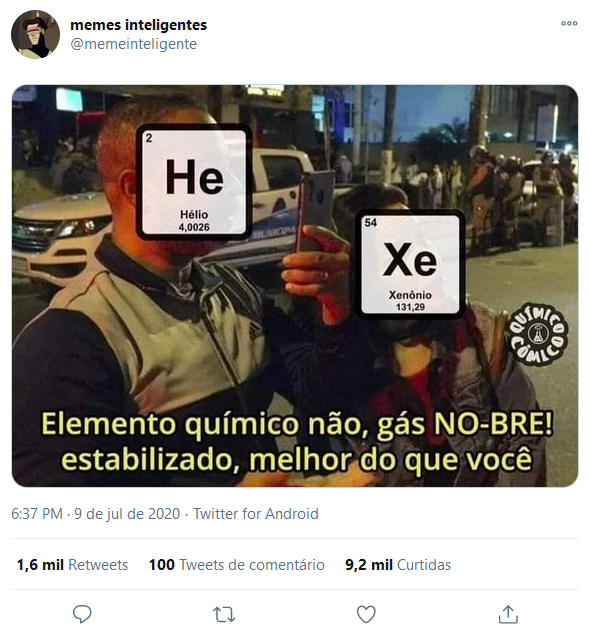
\includegraphics[width=0.5\textwidth]{Fig2.png}
 \caption{\textit{Tweet} do perfil @memeinteligente.}
 \label{fig02}
 \source{Twitter\protect\footnotemark.}
\end{figure}
\footnotetext{Disponível em: \url{https://twitter.com/memeinteligente/status/1281341844933222402}. Acesso em: 24 set. 2020.}

O \textit{tweet} da \Cref{fig02} é formado apenas por uma imagem — não há uma parte escrita no corpo do texto —, que, por sua vez, contém elementos escritos, na cor amarela, na parte inferior, como uma espécie de legenda. Essa configuração textual e a função humorística caracterizam a imagem como um exemplar do gênero meme, que é migrado para o \textit{tweet} do perfil @memeinteligente. É importante acrescentar que a logomarca “químico cômico”, no lado direito da imagem, confirma o pressuposto de \textcite{xavier_desafio_2015} de que a noção de autoria é abalada no hipertexto, uma vez que o perfil @memeinteligente se apropria de uma imagem produzida por outro usuário e a publica em seu perfil.

A imagem original, que serviu de base para a elaboração do meme, é oriunda de uma reportagem\footnote{Disponível em: \url{https://g1.globo.com/fantastico/noticia/2020/07/05/fiscais-sofrem-ataques-ao-reprimir-aglomeracoes-em-bares-do-rio-veja-flagrantes.ghtml}. Acesso em: 20 fev. 2021.} do programa de televisão \textit{Fantástico}, da Rede Globo, que foi ao ar no dia 5 de julho de 2020, isto é, quatro dias antes da postagem do \textit{tweet}. Nessa reportagem, cujo tema foi a fiscalização de aglomeração em bares no Rio de Janeiro durante a pandemia de Covid-19, é mostrada uma discussão entre um casal — que aparece na imagem, sem máscara — e um fiscal de vigilância. Em determinado momento, após ouvir o fiscal tentar apaziguar a situação com a fala “tá, cidadão”, a mulher respondeu: “Cidadão, não. Engenheiro civil, formado. Melhor do que você”. A situação logo viralizou nas redes sociais e gerou diversos memes, a exemplo do mostrado no \textit{tweet} da \Cref{fig02}.

Em uma análise \textit{stricto sensu} do \textit{tweet} publicado por @memeinteligente, é possível notar a presença de intertextualidade temática, estilística e implícita. A intertextualidade temática ocorre por meio do uso de terminologia específica da área de Química, evidenciado nas expressões “elemento químico”, “gás nobre” e “estabilizado”, bem como na imagem dos elementos Hélio e Xenônio, tais como aparecem na tabela periódica, mostrada na \Cref{fig03}:

\begin{figure}[htbp]
 \centering
 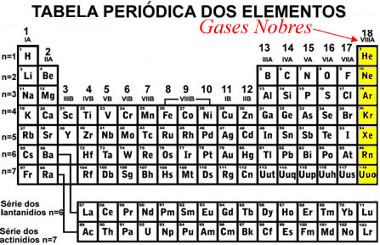
\includegraphics[width=0.75\textwidth]{Fig3.png}
 \caption{Tabela periódica.}
 \label{fig03}
 \source{\textcite{fogaca_gases_nodate}\footnotemark.}
\end{figure}
\footnotetext{Disponível em: \url{https://brasilescola.uol.com.br/quimica/gases-nobres.htm}. Acesso em: 21 fev. 2021.}

Para a compreensão desse (hiper)texto, portanto, é necessário que o leitor conheça a tabela periódica e a classificação de (pelo menos) dois elementos químicos específicos — localizados no 18º grupo da tabela, destacado de amarelo — como “gases nobres”, uma vez que são encontrados em forma gasosa em temperatura ambiente e apresentam estabilidade e pouca reatividade, como aponta \textcite{fogaca_gases_nodate}. Essas informações são ativadas no \textit{tweet} da \Cref{fig02}, que apresenta a imagem dos elementos químicos Hélio e Xenônio e a informação de que eles são gases nobres e estabilizados.

A intertextualidade estilística é observável na paródia da fala da mulher na entrevista supracitada: a frase original “Cidadão, não. Engenheiro civil, formado. Melhor do que você” é transformada em “Elemento químico não, gás NO-BRE! estabilizado, melhor do que você”. Assim, são mantidos elementos do estilo do intertexto, não apenas a nível verbal, uma vez que a imagem da entrevista também é parodiada, quando os elementos químicos Hélio e Xenônio são colocados no lugar do rosto das pessoas que aparecem na reportagem. Além disso, a fonte usada na legenda da imagem apresenta o mesmo estilo de fontes geralmente usadas em legendas de reportagens televisivas. Dessa forma, no \textit{tweet} da \Cref{fig02}, a intertextualidade estilística com um texto audiovisual (a reportagem) se manifesta por meio do uso de recursos multimodais — imagem das pessoas mostradas na reportagem, ilustração dos elementos da tabela periódica e trecho verbal escrito, na cor amarela, com uma espécie de legenda — que contribuem para a construção da paródia.

Além disso, ainda na análise em sentido restrito, observamos que não há menção explícita aos textos-fonte — a tabela periódica e a reportagem do Fantástico. Portanto, o leitor precisa acionar seu conhecimento de mundo para reconhecer os dois textos: a imagem das pessoas, acompanhada da legenda — cujo estilo se assemelha à fala da mulher na reportagem —, e a menção imagética e verbal aos elementos químicos. Por isso, classificamos o tweet da \Cref{fig02} como um caso de intertextualidade implícita, visto que, embora haja pistas visuais e verbais do texto-fonte, não se faz uma referência explícita a ele.

Outro tipo de intertextualidade encontrada nesse hipertexto é a intergenérica, visto que o \textit{tweet} contém um texto do gênero meme e incorpora sua função, qual seja, causar humor, por meio de uma crítica. Com isso, a intergenericidade ocorre porque a forma do \textit{tweet} — socialmente reconhecível pelos falantes, por conta de sua competência metagenérica — é usada com o propósito humorístico do meme, cujo estilo e conteúdo temático são transferidos para o \textit{tweet}. Além disso, em sentido mais amplo, ressaltamos os elementos que assemelham a imagem do \textit{tweet} a reportagens, de modo geral, o que é marcado, por exemplo, pela legenda na cor amarela.

É importante ressaltar que os recursos disponibilizados no hipertexto são essenciais para o enriquecimento do fenômeno de intertextualidade nesse tweet, principalmente a convergência de linguagens, visto que os diferentes tipos de intertextualidade encontrados não ocorrem somente a nível verbal escrito, mas também envolvem outras linguagens, como a visual. O mesmo ocorre nos outros tweets analisados, mostrados mais adiante. 

A seguir, dando prosseguimento à análise de dados, exibimos um tweet postado, no dia 4 de agosto de 2020, pelo perfil @FilosofiaMderna, cujos tweets são relacionados à área de Filosofia, que integra as Ciências Humanas.

\begin{figure}[htbp]
 \centering
 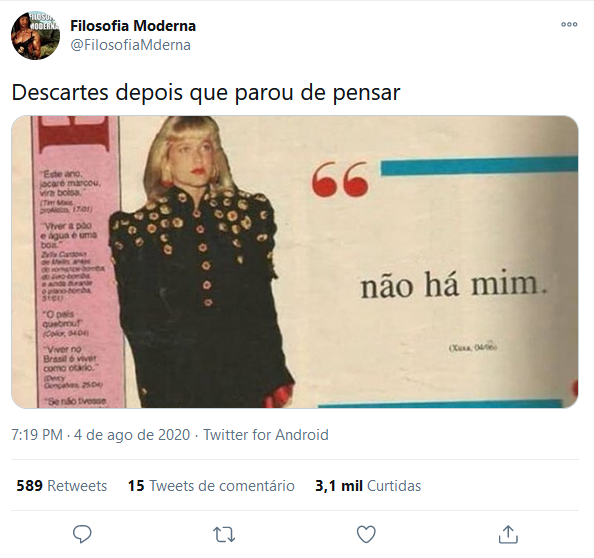
\includegraphics[width=0.5\textwidth]{Fig4.png}
 \caption{\textit{Tweet} do perfil @FilosofiaMderna.}
 \label{fig04}
 \source{Twitter\protect\footnotemark.}
\end{figure}
\footnotetext{Disponível em: \url{https://twitter.com/FilosofiaMderna/status/1290774366762995713}. Acesso em: 15 set. 2020.}

O \textit{tweet} da \Cref{fig04} apresenta um trecho escrito — “Descartes depois que parou de pensar” —, acompanhado por uma imagem que contém uma foto da apresentadora, atriz e cantora Xuxa Meneghel, seguida da citação “não há mim”. A origem dessa imagem, que teve o trecho escrito modificado no \textit{tweet}, está em uma edição de 1992 da revista \textit{Contigo!}, a qual destacava, na seção Frases, a seguinte fala da artista: “No Brasil não há homem para mim”, Esse trecho da revista, assim como a reportagem retratada na \Cref{fig02}, viralizou na internet recentemente e gerou diversos memes. Na \Cref{fig05}, a seguir, mostramos a imagem original: 

\begin{figure}[htbp]
 \centering
 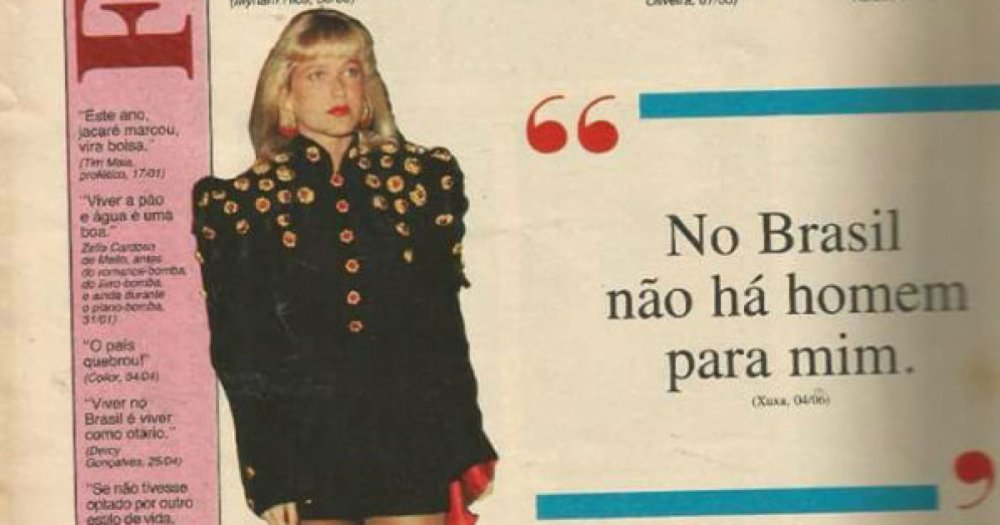
\includegraphics[width=0.5\textwidth]{Fig5.png}
 \caption{Trecho da seção Frases da Revista \textit{Contigo!}.}
 \label{fig05}
 \source{Estadão\protect\footnotemark.}
\end{figure}
\footnotetext{Disponível em: \url{https://cultura.estadao.com.br/galerias/geral,pagina-rara-da-revista-contigo-traz-frases-polemicas-de-famosos-e-bomba-nas-redes-sociais,28236}. Acesso em: 20 fev. 2021.}

Logo de início, é possível observar que, na parte escrita do \textit{tweet} da \Cref{fig04}, há intertextualidade temática com o pensamento do filósofo francês René Descartes, exposto na famosa frase “Penso, logo existo”, identificável por meio da menção explícita ao pensador, mas não à frase, que é recuperada implicitamente, a partir dos conhecimentos de mundo do leitor. Com isso, constatamos a presença de intertextualidade temática com a área de Filosofia, o que condiz com o próprio perfil que a publicou, que se propõe a criar \textit{tweets} relacionados a essa área do conhecimento. A intertextualidade temática, no \textit{tweet} da \Cref{fig04}, é explicitada pelo \textit{user} (@FilosofiaMderna) e pelo \textit{nickname} do perfil (Filosofia Moderna), nos quais o termo “Filosofia” é mencionado.

É possível notar, também, que o \textit{tweet} da \Cref{fig04} apresenta intertextualidade estilística com o trecho da revista que publicou a frase de Xuxa (\Cref{fig05}). No \textit{tweet} de @FilosofiaMderna, a frase atribuída a Xuxa, “No Brasil não há homem para mim”, é reformulada para “não há mim”, demonstrando a supressão de algumas palavras. O perfil se apropria do trecho da revista, por meio de intertextualidade estilística, para abordar a filosofia de Descartes. A paródia da frase dita pela artista à \textit{Contigo!} é realizada por @FilosofiaMderna com o objetivo de estabelecer uma relação entre o meme e o famoso pensamento do filósofo: “penso, logo existo”. Como, segundo a legenda, Descartes teria deixado de pensar, ele não existe mais, o que justifica o uso da frase “não há mim”, que funciona como uma espécie de paráfrase da citação atribuída ao filósofo.

Nesse \textit{tweet}, assim como na \Cref{fig02}, a intertextualidade estilística ultrapassa os limites da linguagem verbal, pois a paródia do estilo do texto-fonte é notável principalmente a partir de aspectos visuais: o \textit{layout} da revista, contendo a foto da apresentadora no lado esquerdo e a frase no lado direito, entre duas barras azuis marcadas com aspas vermelhas. Com isso, a imagem de Xuxa, que faz parte do \textit{layout} do intertexto, funciona como uma marca visual que deve ser acionada pelo leitor para a compreensão do meme. Portanto, ao observarmos o \textit{tweet} de forma integral (trecho escrito e imagem), considerando que o sentido do hipertexto é fruto de uma leitura multissensorial \cite{xavier_desafio_2015}, constatamos que a frase “não há mim” não se refere à artista, como no texto original, e sim a Descartes, conforme explicitado no corpo do \textit{tweet}.

A identificação desse intertexto multimodal e da citação específica de Descartes dependem da ativação de conhecimentos de mundo do leitor, visto que tais textos são apresentados no \textit{tweet} de forma implícita. Como mencionamos, a intertextualidade \textit{stricto sensu}, em hipertextos, é identificável a partir de marcas multimodais, o que ocorre, no \textit{tweet} analisado, por meio da manutenção do estilo da revista e da menção a um filósofo famoso. É a partir de tais pistas que se constrói a interpretação desse hipertexto.

Além disso, observamos, no \textit{tweet} da \Cref{fig04}, uma intergenericidade com o gênero meme, que é formado pela alteração no trecho da revista, acompanhado pela legenda escrita, com o intuito de provocar humor. Ressaltamos que, conforme \textcite{testa_uma_2020}, é comum que os memes apresentem, em sua composição, personagens consagrados, o que inclui personalidades famosas, a exemplo de Xuxa. Então, assim como na \Cref{fig02}, a construção composicional do gênero \textit{tweet} é usada a serviço do conteúdo temático e estilo de um texto no gênero meme, com o qual o \textit{tweet} apresenta intertextualidade intergenérica. Em sentido mais amplo, podemos destacar, ainda, a semelhança da imagem do \textit{tweet} com o gênero do texto-fonte, nomeado por \textcite{pedrosa_frases:_2010} de frases, o qual está presente, de modo geral, em revistas.

Em uma breve comparação entre os \textit{tweets} da \Cref{fig02} e \Cref{fig04}, constatamos que as áreas do conhecimento — Química e Filosofia, respectivamente — se manifestam por meio da intertextualidade temática, ao passo que a intertextualidade estilística se dá de forma multimodal, com textos populares na internet (memes). Esse fato faz com que haja, ainda, manifestação da intertextualidade intergenérica, que une a forma do \textit{tweet} à função do meme. Vejamos, agora, a análise de mais dois \textit{tweets} de cunho didático, nos quais a função humorística não se sobressai.

A seguir, na \Cref{fig06}, apresentamos um \textit{tweet} publicado, em 3 de abril de 2020, pelo usuário @ProfessorNoslen, professor de Língua Portuguesa e “detentor do maior canal de ensino de LP do mundo no YouTube”, como aponta na biografia de seu perfil\footnote{Disponível em: \url{https://twitter.com/ProfessorNoslen}. Acesso em: 15 fev. 2021.}.

\begin{figure}[htbp]
 \centering
 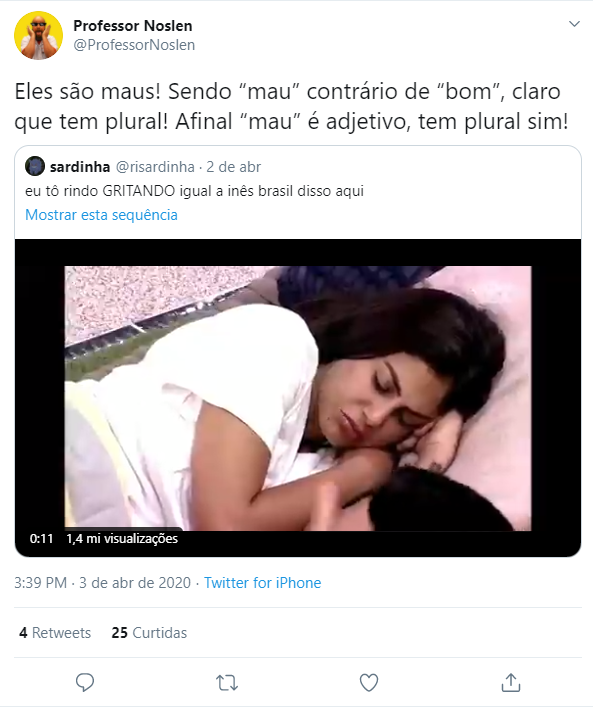
\includegraphics[width=0.65\textwidth]{Fig6.png}
 \caption{\textit{Tweet} do perfil @ProfessorNoslen.}
 \label{fig06}
 \source{Twitter\protect\footnotemark.} 
\end{figure}
\footnotetext{Disponível em: \url{https://twitter.com/ProfessorNoslen/status/1246145341692481536}. Acesso em: 29 ago. 2020.}

O \textit{tweet} da \Cref{fig06} apresenta um retweet comentado, isto é, um compartilhamento de outro tweet, publicado por @risardinha, acompanhado de um comentário próprio do usuário @ProfessorNoslen. O \textit{tweet}-fonte contém um vídeo de uma conversa entre duas participantes da vigésima edição do \textit{reality show} Big Brother Brasil (BBB), no qual elas se questionam se existe plural para a palavra “mau” e “testam” algumas construções linguísticas, como “eles são maus”, “eles são mau” e “são pessoas mau”. O vídeo foi publicado em um \textit{tweet} do perfil @risardinha, acompanhado pela legenda “eu tô rindo GRITANDO igual a inês brasil disso aqui”. @ProfessorNoslen, por sua vez, fez um \textit{retweet} com comentário, no qual elucida a dúvida levantada no vídeo do \textit{reality show}, explicando que a palavra “mau”, por ser um adjetivo, tem plural.

Por meio da construção composicional do \textit{tweet} mostrado na \Cref{fig06}, já é possível identificar uma intertextualidade explícita entre o \textit{tweet} com o vídeo das participantes do BBB e o \textit{tweet} do professor de Língua Portuguesa, cuja publicação é uma espécie de resposta à dúvida levantada no vídeo, linkado ao \textit{tweet} por meio da ferramenta de \textit{retweet} comentado, própria da rede social Twitter. Vemos, assim, que o Twitter, ao materializar esse hipertexto, possibilita uma nova forma de intertextualidade explícita, a saber, a \textit{linkagem} direta do texto-fonte.

Para além disso, observamos uma intertextualidade temática com a área de Língua Portuguesa, marcada pelo uso de terminologia específica, como as palavras “adjetivo” e “plural”, próprias dos estudos de gramática. A relação com a disciplina se dá de forma implícita, uma vez que o usuário @ProfessorNoslen não menciona a fonte da informação a respeito do plural do adjetivo “mau” — provavelmente alguma gramática normativa —, o que é uma característica dos textos didáticos, que, muitas vezes, não explicitam a autoria das ideias apresentadas. Com isso, o \textit{tweet} da \Cref{fig06} é caracterizado, também, por uma intertextualidade estilística, visto que o \textit{tweet} publicado pelo perfil do professor alude ao estilo de textos do campo escolar.

Para finalizar nossa análise, exibimos um \textit{tweet} que pertence à área de Matemática, publicado, no dia 21 de julho de 2020, no perfil da plataforma de ensino online @saladosaberofc, que faz postagens relacionadas a conteúdos de diferentes áreas do conhecimento:

\begin{figure}[htbp]
 \centering
 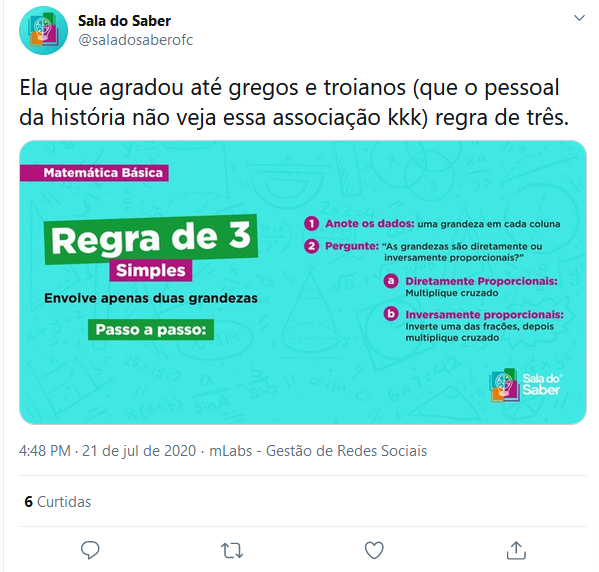
\includegraphics[width=0.65\textwidth]{Fig7.png}
 \caption{\textit{Tweet} do perfil @saladosaberofc.}
 \label{fig07}
 \source{Twitter\protect\footnotemark.}
\end{figure}
\footnotetext{Disponível em: \url{https://twitter.com/saladosaberofc/status/1285663014016909314}. Acesso em: 29 ago. 2020.}

O \textit{tweet} da \Cref{fig07} é formado por uma parte escrita — “Ela que agradou até gregos e troianos (que o pessoal da história não veja essa associação kkk) regra de três.” — e uma imagem, que explica, de modo conciso, a operação matemática conhecida como regra de 3. Nessa imagem, com um fundo azul — que contém ilustrações de figuras geométricas, conjuntos numéricos e outros elementos relacionados à Matemática — e trechos escritos nas cores verde, branco, rosa e preto, explica-se como aplicar a regra de 3 simples, envolvendo apenas duas grandezas, que podem ser diretamente proporcionais ou inversamente proporcionais, o que determina a forma como a regra deve ser usada. No canto direito inferior da imagem, há, ainda, o logotipo da plataforma \textit{Sala do Saber}, formado por três das cores presentes na imagem, de modo que a intertextualidade com a marca \textit{Sala do Saber} é estabelecida por meio do logotipo e, também, do uso das cores.

Nesse \textit{tweet}, é explicitada uma intertextualidade temática com um conteúdo específico da área de Matemática: a regra de 3. Essa relação é mencionada tanto na parte escrita do \textit{tweet}, em que há alusão ao assunto específico, quanto na imagem presente nele, na qual são citados a área de conhecimento e o conteúdo, além de haver utilização de termos específicos da Matemática, como “grandeza”, “diretamente proporcionais”, “inversamente proporcionais”, “frações” e “multiplique”. Apesar de a intertextualidade com o assunto e a área do conhecimento serem apresentados explicitamente, a fonte das informações não é mencionada, o que, como já afirmamos, é uma característica de textos didáticos. Esse aspecto em específico representa uma intertextualidade implícita.

É válido ressaltar, no entanto, que, segundo \textcite{koch_intertextualidade:_2012}, deve-se considerar a explicitude em um contínuo, de modo que há graus maiores e menores, e não apenas textos explícitos ou implícitos, como reforçado por \textcite{mozdzenski_intertextualidade_2013}. Com base nisso, notamos que o \textit{tweet} da \Cref{fig07} apresenta um grau de explicitude maior que o \textit{tweet} da \Cref{fig02}, por exemplo, uma vez que há menção à área do conhecimento com a qual o \textit{tweet} se relaciona — Matemática. Além disso, o conteúdo específico dessa área  — regra de três — também é apontado no \textit{tweet} da \Cref{fig06}, o que o torna mais explícito que o \textit{tweet} da \Cref{fig04}, no qual apenas a área de conhecimento — Filosofia — é indicada. Em comparação com o \textit{tweet} da \Cref{fig06}, porém, o grau de explicitude do \textit{tweet} da \Cref{fig07} é menor, uma vez que @ProfessorNoslen apresenta um link direto para o texto com o qual seu \textit{tweet} se relaciona, o que não ocorre no \textit{tweet} de @saladosaberofc.

Na análise do \textit{tweet} da \Cref{fig07}, constatamos, ainda, que o estilo do trecho escrito do \textit{tweet} se assemelha a uma apresentação, em que comumente se usa um pronome pessoal de terceira pessoa  — “ela” —, acompanhado por uma oração subordinada adjetiva — “que agradou até gregos e troianos” — e seguido pelo referente, isto é, pelo objeto da apresentação — “regra de três”. Assim, constatamos, também, uma ocorrência de intertextualidade estilística.

Além disso, é importante acrescentar que a imagem do \textit{tweet} constitui um exemplar do gênero mapa conceitual, cuja função é sumarizar, por meio de diferentes elementos gráficos, informações a respeito de determinados conceitos e suas conexões \cite{sturm_o_2019} — neste caso, da regra de 3. Trata-se, então, de um caso de intertextualidade intergenérica, visto que o mapa conceitual é integrado ao \textit{tweet}, mantendo sua função de sintetizar objetos de ensino-aprendizagem por meio de ramificações de um conceito principal, funcionando, conforme \textcite{sturm_o_2019}, como uma ferramenta de apoio à aprendizagem. Com isso, o conteúdo temático do mapa conceitual é mantido no \textit{tweet} analisado, cujo objetivo é apresentar, de modo conciso, um conceito da área de Matemática. É importante acrescentar que o gênero mapa conceitual já implica a multimodalidade, visto que as relações entre conceitos e subconceitos são estabelecidas por meio de balões de texto, setas, cores, entre outros elementos verbo-visuais \cite{sturm_o_2019}.

Na parte escrita do \textit{tweet}, há, ainda, intertextualidade implícita com um ditado popular — “agradar gregos e troianos” —, que, por sua vez, apresenta intertextualidade temática com a área de História, visto que se refere à chamada Guerra de Troia, disputada contra a Grécia, entre os anos 1.300 e 1.200 a.C. Esse ditado é retomado com a função de fazer uma espécie de “propaganda” para a regra de 3, a fim de defender a ideia de que essa operação matemática agrada a todos. Trata-se, portanto, de um \textit{détournement}, visto que @saladosaberofc ativa um ditado popular e o orienta para um novo sentido. Esse fenômeno se realiza por meio de adição de palavras ao ditado, que é reformulado em uma nova situação comunicativa.

\section{Considerações finais}\label{sec-formato}
A análise dos \textit{tweets} de cunho didático mostrou que é comum, nesse \textit{corpus}, a ocorrência de mais de uma categoria de intertextualidade e, também, de intertextualidade com múltiplos textos. Desse modo, foi confirmado o pressuposto de \textcite{araujo_consideracoes_2009} de que o hipertexto possibilita diversos tipos de intertextualidade. Mostramos, no quadro a seguir, uma síntese do que encontramos na análise:

\begin{table}[h]
\centering
\caption{Síntese dos resultados encontrados na análise.}
\label{tbl01}
\small
\begin{tabularx}{\textwidth}{cl*{4}{p{0.17\textwidth}}}
\toprule
 & & @memeinteligente & @FilosofiaMderna & @ProfessorNoslen & @saladosaberofc \\
\midrule

\parbox[t]{2mm}{\multirow{5}{*}{\rotatebox[origin=c]{90}{\textit{Stricto sensu}\hspace{9em}}}} & Temática & Área de Química (Ciências Naturais) & Área de Filosofia (Ciências Humanas) & Área de Língua Portuguesa (Linguagens) & Área de Matemática \\
 
 & Estilística & Reportagem do programa de TV \textit{Fantástico} & Trecho da revista \textit{Contigo!} & Textos didáticos & Apresentação;  Textos didáticos \\

 & Explícita & --- & Filósofo Descartes & Tweet com vídeo de participantes do BBB, linkado & Área de Matemática e  regra de 3 \\

 & Implícita & Tabela periódica e reportagem do Fantástico & Trecho da revista \textit{Contigo!};  Famosa citação de Descartes & Gramática da língua portuguesa & Fonte da informação sobre a regra de 3; Ditado popular \\

 & Détournement & --- & --- & --- & Acréscimo de palavras em um ditado popular, com mudança de sentido \\
\arrayrulecolor[gray]{.7}\midrule\arrayrulecolor[gray]{.7}
 & Intergenérica & Gênero meme & Gênero meme & --- & Gênero mapa conceitual \\
 
 \bottomrule
\end{tabularx}
\source{Elaboração própria.}
\end{table}

Tendo em vista a \Cref{tbl01}, fruto da nossa análise de dados, concluímos que a intertextualidade temática com assuntos de diferentes áreas do conhecimento foi identificada em todos os \textit{tweets}, o que está associado com a própria seleção do corpus, visto que consideramos a relação com diferentes áreas do conhecimento para a escolha dos (hiper)textos analisados. Desse modo, o uso de terminologias específicas das áreas de Química, Língua Portuguesa e Matemática, nos \textit{tweets} de @memeinteligente @ProfessorNoslen e @saladosaberofc, e a menção a um importante estudioso da área de Filosofia, no caso do \textit{tweet} de @FilosofiaMderna, demonstraram a produtividade da intertextualidade temática em \textit{tweets} de cunho didático.

Por sua vez, a intertextualidade estilística com textos populares na internet também foi encontrada, em especial nos dois primeiros \textit{tweets}, ao passo que o \textit{détournement} de um ditado popular se manifestou no quarto \textit{tweet}. Exceto pelo hipertexto de @ProfessorNoslen, que produziu um \textit{tweet} em resposta a um vídeo específico, \textit{linkado} ao seu texto, a menção à fonte dos \textit{tweets} — tanto em relação à informação didática quando aos textos populares na internet — não foi explicitada. Ressaltamos, então, que a identificação desses elementos depende da ativação da memória dos leitores, que, dentro de determinado contexto sócio-histórico-cultural, devem reconhecer os intertextos para apreender o sentido dos \textit{tweets}. Consideramos, ainda, que a não menção à origem da informação didática pode ser uma característica do hipertexto, já que as noções de autoria são diferentes nesse modo de enunciar, como comenta \textcite{xavier_desafio_2015}. Trata-se, ainda, de um aspecto comum em textos didáticos, cujo foco está na ideia e não na fonte dela.

Portanto, observamos que a intertextualidade stricto sensu se mostra, nos \textit{tweets} analisados, por meio de \textit{hiperlinks}, representados pelas imagens que constituem os \textit{tweets} das \Cref{fig02}, \Cref{fig04}, \Cref{fig07} e pelo \textit{retweet} comentado no \textit{tweet} da \Cref{fig06}. No entanto, nossa análise confirmou o pressuposto de \textcite{araujo_consideracoes_2009} de que a intertextualidade, nos hipertextos, vai muito além do mero uso de \textit{hiperlinks}, uma vez que o fenômeno, por ser constitutivo da linguagem humana, apareceu de modo produtivo no gênero \textit{tweet}, de diversas maneiras.

Foram encontradas, ainda, ocorrências de intertextualidade intergenérica com o gênero meme, nos \textit{tweets} de @memeinteligente e @FilosofiaMderna, e com o gênero mapa conceitual, no \textit{tweet} de @saladosaberofc. Nesses casos, a construção composicional do \textit{tweet} é unida ao estilo e conteúdo temático desses gêneros, mantendo sua função de causar humor e sintetizar conteúdos programáticos, respectivamente. Além disso, provavelmente por conta do espaço limitado, a intertextualidade tipológica não foi produtiva no corpus observado, o que nos levou a não apresentar essa categoria no \Cref{tbl01}.

Em uma análise lato sensu, além do que já mencionamos, podemos concluir que o hipertexto, em consonância com o suporte Twitter, amplia as possibilidades de intertextualidade, principalmente por conta da viabilidade de coocorrência de várias mídias nos hipertextos do gênero \textit{tweet}. Em todos os \textit{tweets} analisados neste artigo, o fenômeno de intertextualidade se manifesta a partir da multimodalidade, isto é, da convergência de linguagens e mídias, que funcionam como uma espécie de alicerce para a enunciação de um objetivo didático. Concluímos, então, que o gênero \textit{tweet} apresenta um alto grau de intertextualidade e que esse fenômeno ocorre de forma multissemiótica.

Com base nisso, consideramos que o gênero \textit{tweet} pode ser abordado em sala de aula, conforme sugere a Base Nacional Comum Curricular \cite{brasil_base_2018}, ao orientar os docentes para o uso de tecnologias digitais na escola. Desse modo, propostas didáticas voltadas para a intertextualidade de \textit{tweets} cumpririam o papel de proporcionar um ensino interdisciplinar e mais próximo de usos autênticos da linguagem, visto que, como mostramos em nossa análise, os \textit{tweets} de cunho didático dialogam com vários textos e com várias linguagens presentes na sociedade. Assim, o trabalho com textos como os que apresentamos neste artigo contribuiria para o letramento dos estudantes, que aprenderiam a lidar, de modo mais sistematizado, com um gênero digital — o \textit{tweet} —, com a multimodalidade e com o fenômeno de intertextualidade, constitutivo da linguagem humana.

\printbibliography\label{sec-bib}
% if the text is not in Portuguese, it might be necessary to use the code below instead to print the correct ABNT abbreviations [s.n.], [s.l.] 
%\begin{portuguese}
%\printbibliography[title={Bibliography}]
%\end{portuguese}

%full list: conceptualization,datacuration,formalanalysis,funding,investigation,methodology,projadm,resources,software,supervision,validation,visualization,writing,review
\begin{contributors}[sec-contributors]
\authorcontribution{Ana Claudia Oliveira Azevedo}[conceptualization,datacuration,investigation,projadm,visualization,writing]
\authorcontribution{Márcia Helena de Melo Pereira}[conceptualization,supervision,review]
\end{contributors}

\end{document}
